\chapter{Realisieren}\label{ch:realisieren}
Dieses Kapitel zeigt die in der IPERKA-Phase «Realisieren» durchgeführten Arbeiten auf. In dieser Phase wird beschrieben wie der Lernende die Aufgabe umgesetzt hat und spricht Probleme bei der Umsetzung an.

\section{Endpoints für die Mindestanforderungen erstellen}
Die Reihenfolge, welche für diesen Abschnitt folgt, ist die Reihenfolge in der Implementiert wurde.

\subsection{MqInDTO}
Die Implementierung wurde mit der Erstellung von der MqInDto.java Klasse gestartet. Diese Klasse wird öfter in anderen Klassen verwendet und ist aus diesem Grund ein guter Startpunkt. Sie wurde mithilfe der MqOutDto.java Klasse als Beispiel erstellt, um die Konsistenz zwischen den verschiedenen DTO-Klassen beizubehalten. Sie beinhaltet mehrere Annotationen, um den Code kurzzuhalten und Zeit bei der Implementation zu sparen:

\paragraph{@Data} \footnote{\url{https://projectlombok.org/features/Data}} generiert Getter, Setter und mehr .
\paragraph{@SuperBuilder} \footnote{\url{https://projectlombok.org/features/experimental/SuperBuilder}} erstellt ein Builder, welcher auch Felder von einer Superklasse verwenden kann.
\paragraph{@NoArgsConstructor} \footnote{\url{https://projectlombok.org/features/constructor}} generiert einen Konstruktor ohne Parameter.
\paragraph{@Schema} \footnote{\url{https://www.baeldung.com/swagger-parameter-vs-schema}} für die Kontrolle von spezifischen Definitionen wie Beschreibung oder Beispiele.
\paragraph{@NotNull} \footnote{\url{https://www.baeldung.com/java-notnull-method-parameter}} stellt sich, dass das Feld nicht «null» ist.\newline

\noindent Anschliessend wurden die Felder erstellt, mit den oben entsprechenden genannten Annotationen, die für die Tabelle im Frontend genutzt werden.

\subsection{MqInMapper}
Die Klasse MqInMapper.java hat die Annotation @Component, sodass Springboot diese Klasse instanziieren und sie mit allen angegebenen Abhängigkeiten injizieren kann.

Zwei Funktionen namens toMqInDto() und listToMqInDto() wurden in dieser Klasse erstellt. Die erste Funktion macht ein Mapping von MqTablePC (die ursprüngliche MqInPC-Klasse) zu MqInDto. Sie verwendet den Builder von der zuvor genutzten Annotation @SuperBuilder. Die zweite Funktion ruft die erste mithilfe von einem Stream auf. Der Stream wird verwendet, um jedes Element der Liste mit der Funktion toMqInDto() aufzurufen. Dies wird mit .map() gemacht. Der Stream ermöglicht es, diese Aufgabe in einer kurzen Zeile zu schreiben, anstatt mit einem Loop jedes einzelne Element der Liste hervorzuholen, zu mappen und anschliessend in einer zweiten Liste zu speichern. Die Funktion hat durch das nur insgesamt 3 Zeilen und vereinfacht das lesen.

\begin{verbatim}
	public List<MqInDto> listToMqInDto(List<MqTablePC> listOfMqTablePCs) {
		return listOfMqTablePCs.stream().map(this::toMqInDto).toList();
	}
\end{verbatim}

\subsection{MqInService}
Um die Struktur eines Services vorzugeben, wurde ein Interface mit dem Namen MqInService erstellt. Dieses Interface wird später für die Klasse MqInServiceImpl.java und MqInServiceMockImpl.java verwendet und beinhaltet im Moment zwei Funktionen für das hervorholen von allen MqTables in der Datenbank und das Ausführen von einem neuen Verarbeitungsversuch.

\subsection{MqInServiceImpl}
MqInServiceImpl wird vom Interface MqInService implementiert. Sie wird mit der Annotation @Service für Springboot als Service deklariert. Die Klasse enthält die vom Interface vorgegebene Funktion getMqTables(). Sie ruft eine Funktion von der Klasse MqTableDao (die ursprüngliche MqInDao-Klasse) auf, die alle MqTable Einträge mit dem Status «Error» von der Datenbank hervorholt und sie auf 25 Einträge limitiert. Ein ähnliches Vorgehen hat die Funktion executeNewProcessingAttempt(), die den Status vom MqIn auf NEW setzt.    

In dieser Klasse wurde auch ein Konstruktor erstellt. Bei dieser Implementierung trat ein Problem auf, welches die Applikation nicht starten liess. Bei dem Parameter MqTableDao erschien die Meldung «Could not autowire. No beans of 'MqTableDao' type found.». Das Problem war, dass für die Klasse MqTableDao noch kein Bean erstellt wurde, obwohl die Klasse schon vorher existierte. Das Bean wurde anschliessend in der Klasse WebBackendAdminSpringConfiguration.java erstellt.

\subsection{MqTableDao}
Diese Klasse existierte bereits und war ursprünglich als MqInDao geplant. Durch das mussten nur die Funktionen hinzugefügt werden. Da es ein Interface ist, wurden nur die Namen und die benötigten Parameter hinzugefügt. Es wurden noch keine Bodys implementiert. Ausserdem wurden bei beiden Funktionen ein Kommentar erstellt. Der Kommentar beinhaltet eine kurze Beschreibung der Funktion und was sie zurückgibt. Mithilfe dieses Kommentars kann man jetzt über die Funktion drüberfahren und die Beschreibung wird als kurze Erklärung angezeigt.

\subsection{MqTableHibernateDao}
In der Klasse MqTableHibernateDao wird das Interface MqTableDao implementiert und muss durch das auch die neu erstellte Funktion implementieren.

Die Funktion nutzt einen CriteriaBuilder, um eine SQL-Query zu erstellen. Mit dieser Klasse konnte die Query so generiert werden, dass sie nach Einträgen filtert, die einen MQ\_IN\_STATUS von ERROR, also die Nummer Drei, haben. Die Query wird mithilfe von der Klasse CriteriaQuery bearbeitet und mit der Klasse Root können die einzelnen Spalten hervorgeholt werden, um sie zu vergleichen.

Um die Einträge auf 25 zu limitieren, musste noch die Klasse TypedQuery verwendet werden, welche dies ermöglichte.

\begin{verbatim}
	@Override
	public List<MqTablePC> findAllWithStatusErrorLimitedTo25() {
		CriteriaBuilder cb = getSession().getCriteriaBuilder();
		CriteriaQuery<MqTablePC> query = cb.createQuery(MqTablePC.class);
		Root<MqTablePC> mqTable = query.from(MqTablePC.class);
		
		query.where(
			cb.equal(mqTable.get(FN_MQ_IN_STATUS), ERROR)
		).orderBy(cb.desc(mqTable.get(FN_MODIFIED_AT)));
		
		TypedQuery<MqTablePC> typedQuery = getSession().createQuery(query);
		typedQuery.setMaxResults(25);
		
		return typedQuery.getResultList();
	}
\end{verbatim}

\noindent Für die zweite Funktion wurde ein CriteriaUpdateBuilder verwendet. Die restliche Implementation blieb fast gleich. Die Limitierung wurde entfernt und ein set() hinzugefügt, um den MQ\_IN\_STATUS auf NEW zu setzen.

\subsection{MqInResource}
Die Klasse MqInResource beinhaltet den geplanten Endpoint, welcher im Arbeitspaket \ref{tab:realisieren-4.1} beschrieben wurde. Die Klasse wurde mit @RestController annotiert, sodass Spring weiss das diese Klasse Endpoints enthält. Sie hat ausserdem noch @RequestMapping, um den Pfad zu definieren, und @RequiredArgsConstructor, welcher ein Konstruktor generiert, mit allen finalen und nicht-null Feldern.

Der Endpoint selbst hat drei Annotationen:

\paragraph{@GetMapping} \footnote{\url{https://www.geeksforgeeks.org/spring-postmapping-and-getmapping-annotation/}} deklariert diesen Endpoint als ein GET-Request.
\paragraph{@Operation} \footnote{\url{https://www.baeldung.com/swagger-operation-vs-apiresponse}} beschreibt die Funktion von diesem Endpoint.
\paragraph{@RequirePermission} \footnote{Vom Projekt CardX implementiert} stellt die Befugnis von diesem Endpoint ein. \newline

\noindent Der Endpoint selbst greift nur auf die erstellte Funktion in der Klasse MqInService.java zu und mappt das erhaltene Resultat mithilfe des Mappers bevor er es wieder zurücksendet.

Der zweite Endpoint für das Ausführen von einem weiteren Verarbeitungsversuch ist gleich aufgebaut wie der erste, mit zwei Unterschieden. Er hat zwei andere Annotationen. Einerseits wurde das @GetMapping mit einem @RequestMapping ersetzt, sodass Spring weiss, dass es die Requests zu den richtigen Endpoints verweisen kann. Ausserdem hat dieser Endpoint einen Parameter namens id. Dieser Parameter wird vom Request Body befüllt und muss deshalb mit @RequestBody annotiert werden.

\section{Die Seite und Tabelle im Frontend erstellen}

\subsection{Erstellung der Tabelle}\label{ch:creation-of-table}
Für die Erstellung der Tabelle wurde eine mq-in.service.ts-Klasse erstellt. Diese wird für die Requests an das Backend verwendet und beinhaltet die Funktion getAllMqInsLimitedTo25(), um alle MqIns von der Datenbank zu laden, und executeNewProcessingAttempt(id: number), die für die erneute Ausführung von einem Verarbeitungsversuch zuständig ist. Beide Funktionen rufen ihren erstellten Endpoint auf, welcher für das Frontend des Projekts generiert wurde.

Diese Generierung kann mithilfe der Annotationen bei den entsprechenden Endpoints die HTTP-Requests generieren. Durch die generierte Swagger-Datei wird eine zweite JSON-Datei generiert, die alle benötigten Informationen beinhaltet und im Modul Interface als web-backend-admin-api-.json gespeichert wird. Ein Plugin im Frontend nutzt anschliessend diese Datei, um die HTTP-Requests zu generieren.

Die Generierung vereinfachte die Nutzung von HTTP-Requests und hat die entsprechende Implementierung beschleunigt. Die Tabelle für die MqIns wurde durch das schnell erstellt und die ersten Einträge waren sichtbar auf der Seite.

\begin{figure}[H]
	\begin{center}
		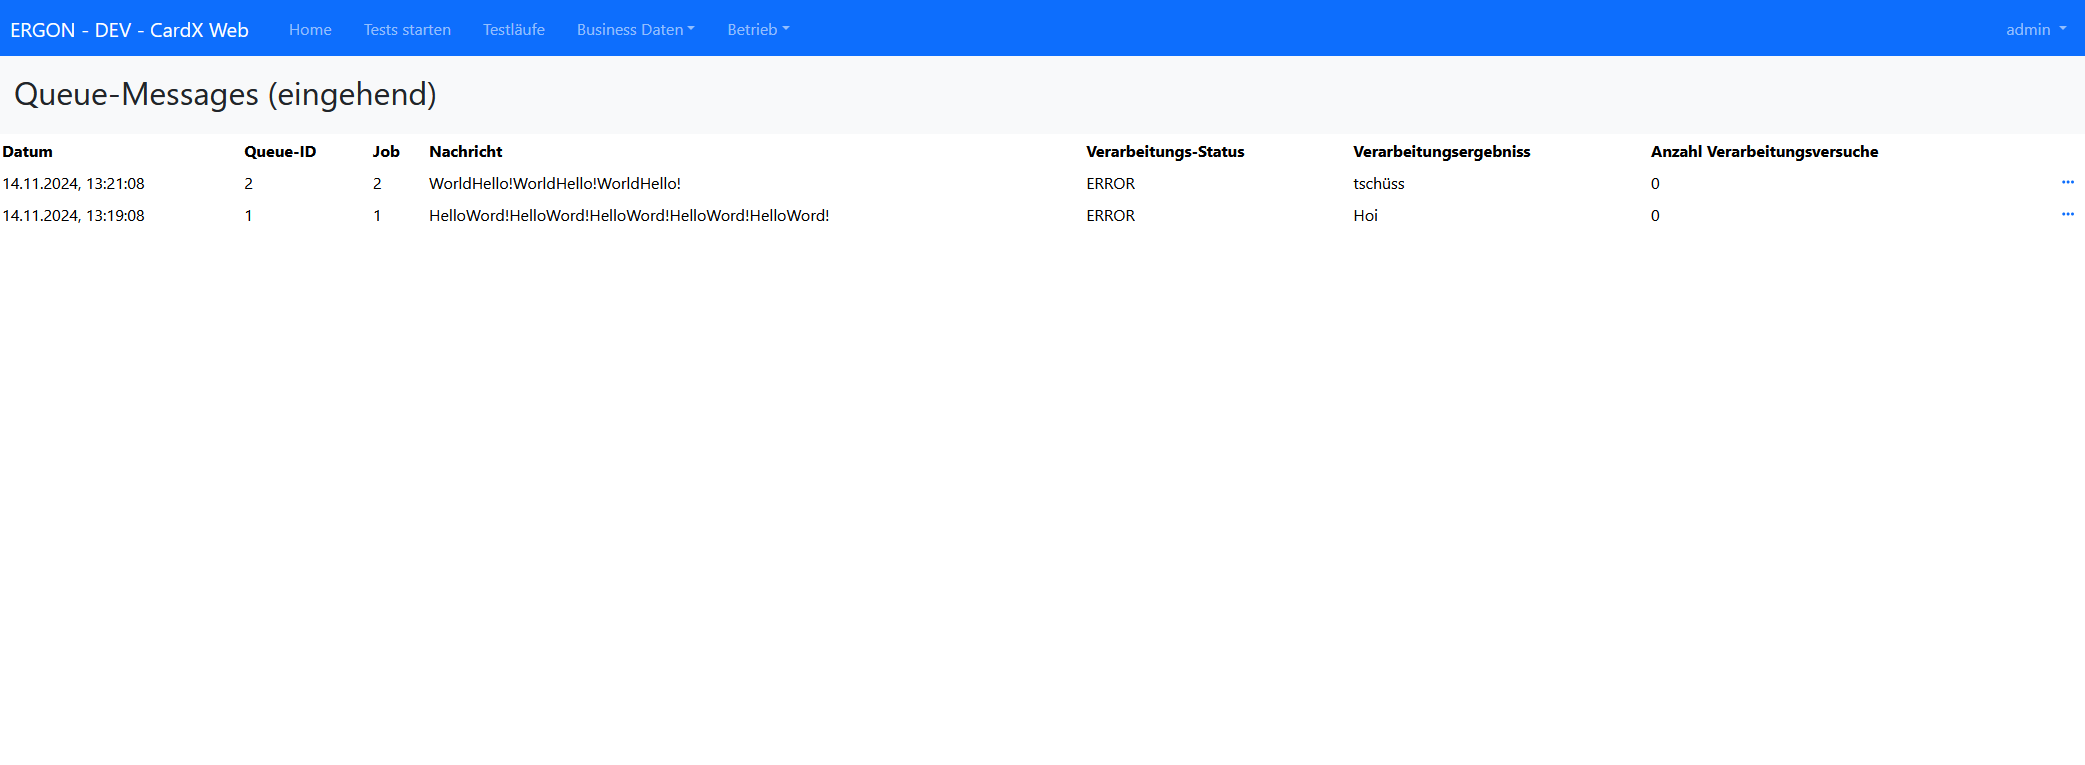
\includegraphics[width=1\textwidth]{ressourcen/4.2_Tabelle}
		\caption[Aktueller Stand der Tabelle]{Aktueller Stand der Tabelle}\label{fig:4.2-tabelle}
	\end{center}
\end{figure}

\subsection{Anzeigen der ganzen Nachricht}
Für das Anzeigen der ganzen Nachricht wurde eine neue Map erstellt, welche als Key die id des MqIns und als Value einen Boolean enthält. Diese Map wird immer beim Aufruf der Seite gefüllt, nach dem die MqIns geladen wurden. Durch diese Map kann die ganze Nachricht angezeigt und anschliessend wieder verkürzt werden. Die eine Funktion setzt den entsprechenden Wert jedes Mal um, wenn man auf den Knopf «ganze Nachricht anzeigen» oder «Nachricht kürzen» drückt.

\noindent Die kurze Nachricht wird angezeigt:
\begin{figure}[H]
	\begin{center}
		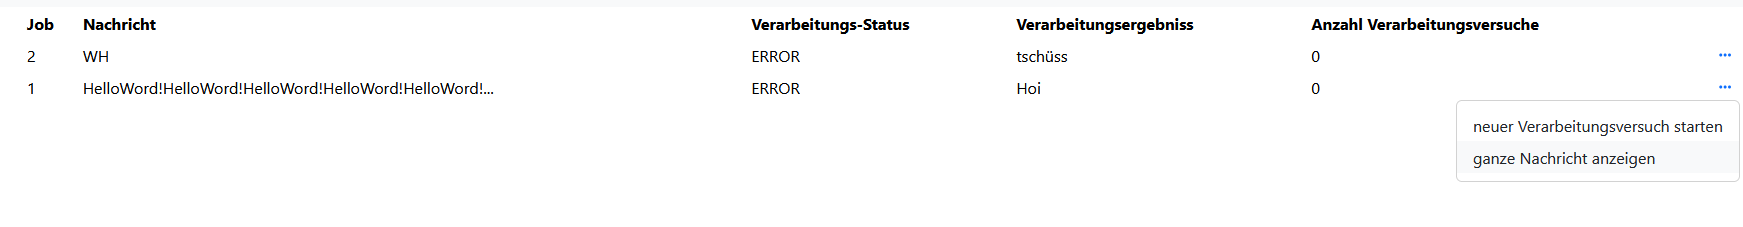
\includegraphics[width=1\textwidth]{ressourcen/Kurze-Nachricht}
		\caption[Gekürzte Nachricht]{Gekürzte Nachricht}\label{fig:show-shortend-version-of-message}
	\end{center}
\end{figure}

\noindent Die ganze Nachricht wird angezeigt:
\begin{figure}[H]
	\begin{center}
		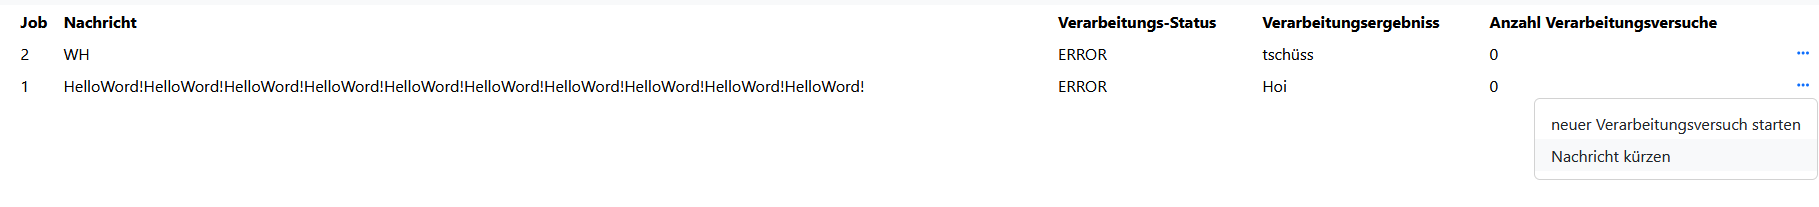
\includegraphics[width=1\textwidth]{ressourcen/Ganze-Nachricht}
		\caption[Ganze Nachricht]{Ganze Nachricht}\label{fig:show-hole-message}
	\end{center}
\end{figure}

\subsection{Erneutes Ausführen vom Verarbeitungsversuch}
Die Implementation für dieses Feature dauerte nicht lange, da, wie oben beschrieben \ref{ch:creation-of-table}, die HTTP-Requests generiert wurden und die Funktion nur noch verknüpft werden musste beim Drücken des Knopfs «neuer Verarbeitungsversuch starten». Dies war schnell gemacht und kostete nur im Backend ein wenig Zeit.

\begin{verbatim}
	private executeNewProcessingAttempt(id: number) {
		this.mqInService.executeNewProcessingAttempt(id)
		.subscribe({
			next: () => {
				this.loadMqIns();
			},
			error: (e: HttpErrorResponse) => {
				throw new ApiHttpErrorResponse('Die Verarbeitung der Queue konnte nicht neu gestartet werden.', e);
			},
		});
	}
\end{verbatim}

\noindent Diese Funktion ruft die Funktion executeNewProcessingAttempt() mit dem Parameter id auf. Anschliessend führt die Subscribe-Funktion folgende zwei Aktionen aus:

\paragraph{next:} wird ausgeführt, wenn der HTTP-Request erfolgreich war und die erwarteten Daten bereitgestellt wurden. In diesem Fall wird die Liste neu geladen.
\paragraph{error:} wird ausgeführt, wenn der HTTP-Request nicht erfolgreich war und ein Fehler während der Ausführung auftrat. Hier wird ein Fehler mit einer Nachricht geworfen.\newline

\noindent Danach ist die Backend-Anfrage fertig und war entweder erfolgreich oder nicht.

\section{Endpoints für die Erweiterung Filter erstellen}
Die Reihenfolge, welche für diesen Abschnitt folgt, ist die Reihenfolge, in der implementiert wurde. Die Klassen werden nicht mehr im Detail beschrieben, was oben bereits erklärt wurde.

\subsection{MqInFilterDto}
Um die Datensätze der Datenbank zu filtern, wurde ein weiteres DTO erstellt, um die Filterkriterien vom Frontend zu empfangen. Die Klasse beinhaltet vier Variablen namens status, messageQuery, timestampFrom und timestampTo. Ausserdem sind alle Variablen noch mit der Annotation @Schema beschrieben.

\subsection{MqInService}
Im Interface MqInService wurde wieder eine neue Funktion, getFilteredMqTablePCs(), hinzugefügt. Sie nimmt einen Parameter mit dem Typ MqInFilterQuery, dieser Record wurde in der Klasse MqTableDao hinzugefügt und wird später nochmals genauer erklärt, und gibt eine Liste mit MqTablePCs zurück.

\subsection{MqInServiceImpl}
Die Implementierung der neu erstellten Funktion im Interface MqInService wurde hier implementiert. Die Funktion hat gerade mal eine Zeile Code, der im Interface MqTableDao eine weitere Funktion aufruft.

\subsection{MqTableDao}
Das Interface hat zwei neue Inhalte dazu bekommen.

Einerseits wurde die neue Funktion getFilteredMqTablePCs() deklariert. Sie hat den gleichen Parameter und Rückgabewert wie die Funktion im Interface MqInService.

Und andererseits wurde hier ein neuer Record namens MqTableFilterQuery hinzugefügt. Ein Record ist eine spezielle Art von Klasse, die hauptsächlich für datenzentrierte Klassen dient. Die Klasse ist dadurch einfach und prägnant, da sie Funktionen wie Konstruktoren, Getter, toStirng, hashCode oder equals bereits implementiert und sie so nicht erneut geschrieben werden müssen. Die Felder der Klasse werden durch Parameter angegeben. Dieser Record beinhaltet status, messageQuery, timestampFrom und timestampTo als Parameter.

\subsection{MqTableHibernateDao}
Die zuvor deklarierte Funktion getFilteredMqTablePCs() wird hier implementiert. Sie hat ähnliche Variablen wie die anderen Funktionen in dieser Klasse, wie CriteriaBuilder, CriteriaQuery und Root. Was bei dieser Funktion speziell ist, sie hat eine weitere Variable mit dem Typ Predicate. Diese Variable ermöglicht es, eine Liste von Filtern zu erstellen. Da nicht immer alle Filter gesetzt werden, müssten ansonsten mehrere Funktionen erstellt werden. Mit dieser Variable kann man die gesetzten Filter zu der Liste hinzufügen und am Ende die Elemente zu der SQL-Query hinzufügen. Dies hat es also ermöglicht, alle Filter mit einer Funktion zu setzen und so das richtige Resultat zu erhalten.

\begin{verbatim}
	@Override
	public List<MqTablePC> getFilteredMqTablePCs(MqTableFilterQuery filterQuery) {
		CriteriaBuilder cb = getSession().getCriteriaBuilder();
		CriteriaQuery<MqTablePC> query = cb.createQuery(MqTablePC.class);
		Root<MqTablePC> mqTable = query.from(MqTablePC.class);
		List<Predicate> predicates = new ArrayList<>();
		
		Optional.ofNullable(filterQuery.status()) // Einfügen der Filters status
		.ifPresent(status ->
		predicates.add(cb.equal(mqTable.get(FN_MQ_IN_STATUS), status))
		);
		
		Optional.ofNullable(filterQuery.messageQuery()) // Einfügen der Filters messageQuery
		.ifPresent(messageQueue -> {
			String searchTerm = "%" + filterQuery.messageQuery().toLowerCase(Locale.getDefault()) + "%";
			predicates.add(
			cb.or(
			cb.like(cb.lower(mqTable.get(FN_MESSAGE_SHORT).as(String.class)), searchTerm),
			cb.like(cb.lower(mqTable.get(FN_MESSAGE_LONG).as(String.class)), searchTerm)
			)
			);
		});
		
		Optional.ofNullable(filterQuery.timestampFrom()) // Einfügen der Filters timestampFrom
		.ifPresent(timestampFrom ->
		predicates.add(cb.greaterThanOrEqualTo(mqTable.get(FN_MODIFIED_AT), timestampFrom))
		);
		
		Optional.ofNullable(filterQuery.timestampTo()) // Einfügen der Filters timestampTo
		.ifPresent(timestampTo ->
		predicates.add(cb.lessThanOrEqualTo(mqTable.get(FN_MODIFIED_AT), timestampTo))
		);
		
		
		query.select(mqTable)
		.where(cb.and(predicates.toArray(Predicate[]::new)))
		.orderBy(cb.desc(mqTable.get(FN_MODIFIED_AT)));
		
		return getSession().createQuery(query)
		.setMaxResults(25)
		.getResultList();
	}
\end{verbatim}

\subsection{MqInResource}
Für den neuen Endpoint in der Klasse MqInResource wurde wieder der gleiche Aufbau genutzt wie bei dem Endpoint executeNewProcessingAttempt(). Die Annotationen sind gleich, ausser die Beschreibung, und der Parameter wird auch mit der Annotation @RequestBody annotiert. Im Inhalt der Funktion wird aber zuerst der Parameter gemappt und erst dann die Funktion getFilteredMqTablePCs() vom Service aufgerufen.

\section{Die Erweiterung in die Tabelle integrieren}
Durch die grosse Verzögerung während des Implementierens von diesem Teil hat sich der Lernende dazu entschieden, die Erweiterung zu pausieren und zuerst mit den restlichen Arbeitspaketen weiter zu machen. Falls am Ende der Probe-IPA noch Zeit übrig ist, wird die Implementierung fortgesetzt.  

Die Reihenfolge, welche für diesen Abschnitt folgt, ist die Reihenfolge in der Implementiert wurde.

\subsection{mq-in-filter-url}
Um die Parameter von der URL für das Filtern zu extrahieren, wurde in dieser Klasse eine Funktion getMqInFilterUrlStateFromParams erstellt. Diese Funktion nimmt eine Map als Parameter. Mit dieser Map wird mithilfe vom Enum MqInFilterUrlKeys alle Werte von der URL hervorgeholt und anschliessend alle Werte, die nichts beinhalten, aus der Liste entfernt. Als Rückgabewert wird MqInFilterUrlState verwendet.

Dieser Typ beinhaltet Keys mit dem Typ MqInFilterUrlKeys und die Werte haben einen Typ String. Dies wird mit einem Record definiert. Durch das Hinzufügen des Typs Partial werden die Werte optional und müssen nicht befüllt werden.

\begin{verbatim}
	export enum MqInFilterUrlKeys {
		STATUS = 'status',
		MESSAGE_QUEUE = 'messageQuery',
		TIMESTAMP_FROM = 'timestampFrom',
		TIMESTAMP_TO = 'timestampTo',
	}
	
	export type MqInFilterUrlState = Partial<Record<MqInFilterUrlKeys, string>>;
	
	export function getMqInFilterUrlStateFromParams(params: ParamMap): MqInFilterUrlState {
		const result: MqInFilterUrlState = Object.values(MqInFilterUrlKeys)
		.reduce((state, urlParam) => ({ ...state, [urlParam]: params.get(urlParam) }), {});
		return omitBy(result, isEmpty);
	}
\end{verbatim}

Anschliessend wurde noch ein Mapping für den Typ FilterQueryDto erstellt für die Backend-Anfrage.

\subsection{mq-in-filter.component}
Diese Klasse wird für das Anzeigen der Filter verwendet. Es wurde ein FormGroup erstellt, mit den Filter-Werten, die anfangs einfach Null sind. Der Status jedoch hat den Wert ERROR, um den Mindestanforderungen gerecht zu werden, da sie bei der ersten Abfrage nur Elemente mit diesem Wert wollen. Dies wird durch ein ngOnInit() gemacht, da diese Funktion immer als erstes ausgeführt wird, wenn man die Seite aufruft.

Um die Werte von der URL in das Formular einzufügen, wurde eine weitere Funktion erstellt, die alle Parameter mit der Hilfe von der zuvor erstellten Funktion getMqInFilterUrlStateFromParams(). Sie speichert die erhaltenen Parameter in einer Variable und setzt anschliessend die FormGroup mit den erhaltenen Werten.

Um eine Filterung durchzuführen, werden beim Event «submit» alle Werte des Filters im Typ MqInFilterUrlState gespeichert und anschliessend für die Elternkomponente durch das Event bereitgestellt

Das Endresultat der implementierten Funktionen und Klassen sieht anschliessend im Web-GUI so aus:

\begin{figure}[H]
	\begin{center}
		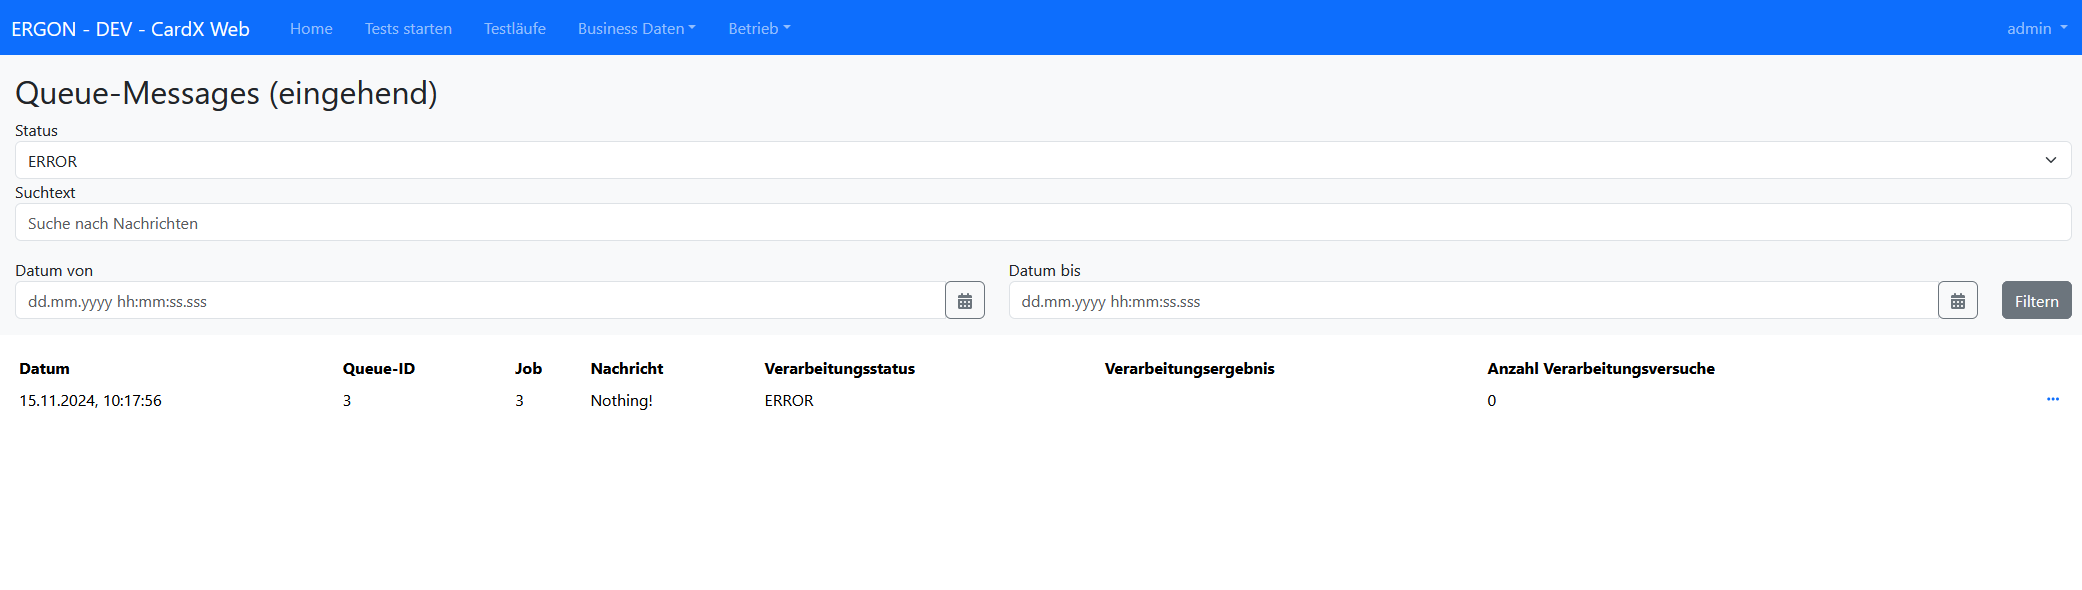
\includegraphics[width=1\textwidth]{ressourcen/Filterung}
		\caption[Der aktuelle Stand des Filters]{Der aktuelle Stand des Filters}\label{fig:filtering-v1}
	\end{center}
\end{figure}

\subsection{Fehlerbeschreibung}
Durch einen Fehler, welcher nicht ermittelt werden konnte, wurde die Erweiterung pausiert. Der Fehler erscheint anfangs beim Aufrufen der Seite und hat den HTTP-Statuscode 500, was auf einen Server-internen Fehler hinweist. Es wurde nicht herausgefunden, was der Fehler war. Mit Debugging wurde versucht, den Request im Backend abzufangen und manuell durch die Funktionen zu gehen, aber der Request kam nicht im Backend an. Nach ein paar Stunden Debugging und Fehlersuche wurde entschieden, dass die Implementation der Erweiterung pausiert wird und zu einem späteren Zeitpunkt erneut ein neuer Versuch gestartet wird, mit einem Fachverantwortlichen.

\subsection{Update des letzten Tages}
Es wurde herausgefunden was der Fehler war. Der erste Request an das Backend wird nicht korrekt befüllt und verursacht durch das fehlgeschlagene Parsen von null einen Fehler. Die Lösung war ein (click)-Event bei dem button zu erstellen und die Funktion onSubmit() auszuführen. Diese Funktion ist aber noch nicht ganz Fehlerfrei und die Zeit fehlt um dies zu beheben.

\begin{verbatim}
	<div class="col-auto">
	    <label class="d-block">&nbsp;</label>
	    <button type="submit" class="btn btn-secondary" (click)="onSubmit()">
	      Filtern
	    </button>
	</div>
\end{verbatim}

\section{ReleaseNotes schreiben}
Um die Änderungen in den Master mergen zu können, muss man Release Notes für das implementierte Jira-Ticket schreiben. Für dieses Ticket wurden folgende Release Notes geschrieben:

\begin{verbatim}
	## Webinterface
	* CARDXDEV-2268 Neue Seite unter Business Daten > Queue Messages (eingehend)
	  hinzugefügt mit einer MqIn-Tabelle.
\end{verbatim}
\newpage